\documentclass[a4paper, 12pt]{article}%тип документа

%отступы
\usepackage[left=2cm,right=2cm,top=2cm,bottom=3cm,bindingoffset=0cm]{geometry}

%Русский язык
\usepackage[T2A]{fontenc} %кодировка
\usepackage[utf8]{inputenc} %кодировка исходного кода
\usepackage[english,russian]{babel} %локализация и переносы

%Вставка картинок
\usepackage{wrapfig}
\usepackage{graphicx}
\graphicspath{{pictures/}}
\DeclareGraphicsExtensions{.pdf,.png,.jpg}

%оглавление
\usepackage{titlesec}
\titlespacing{\chapter}{0pt}{-30pt}{12pt}
\titlespacing{\section}{\parindent}{5mm}{5mm}
\titlespacing{\subsection}{\parindent}{5mm}{5mm}
\usepackage{setspace}

%Графики
\usepackage{multirow}
\usepackage{pgfplots}
\pgfplotsset{compat=1.9}

%Математика
\usepackage{amsmath, amsfonts, amssymb, amsthm, mathtools}

%Заголовок
\author{Валеев Рауф Раушанович\\
группа 825}
\date{}
\title{\textbf{Работа 5.1.3\\Изучение рассеяния медленных электронов на атомах (эффект Рамзауэра)}}
\newtheorem{task}{Задача}
\begin{document}
\maketitle
\newpage
\paragraph*{Цель работы: } Получить ВАХ эффекта на экране ЭО, измерить расстояния между характерными точками в вольтах; снять ВАХ в статическом режиме; по результатам измерений рассчитать размер электронной оболочки атома, оценить глубину потенциальной ямы и потенциал ионизации газа, заполняющего лампу.
\section*{Теория}
\subsection*{Эффект Рамзауэра}
\textit{Эффективное сечение реакции} --- это величина, характеризующая вероятность перехода системы двух сталкивающихся частиц в результате их рассеяния (упругого или неупругого) в определенное конечное состояние. Сечение $\sigma$ это отношение числа таких переходов $N$ в единицу времени к плотности потока $nv$ рассеиваемых частиц, падающих на мишень, т.е. к числу частиц, падающих в единицу времени на единичную площадку, перпендикулярно к их скорости.

\begin{equation}
\sigma = \frac{N}{nv}
\end{equation}

Эффект Рамзауэра нельзя объяснить с позиции классической теории. С квантовой же точки зрения картина рассеяния выглядит следующим образом: внутри атома потенциальная энергия падающего электрона отлична от нуля, скорость электрона меняется, становясь равной $v'$ в соответствии с законом сохранения энергии 

\[E = \frac{mv^2}{2} = \frac{mv'^2}{2}+U\]

а значит, изменяется и длина его волны де-Бройля. Таким образом, по отношению к электронной волне атом ведет себя как преломляющая среда с относительным показателем преломления
\begin{equation}
n = \frac{\lambda}{\lambda'} = \sqrt{1 - \frac{U}{E}}
\end{equation}

Решение задачи о рассеянии электрона на сферическом потенциале достаточно громоздко. Поэтому рассматривают более простое одномерное приближение: электрон рассеивается на потенциальной яме конечной глубины. После решения соответствующего уравнения Шрёдингера получается выражение для коэффициента прохождения:

\begin{equation}
D = \frac{16 k_1^2 k_2^2}{16k_1^2 k_2^2 + 4\left(k_1^2-k_2^2\right)^2\sin^2\left(k_2 l\right)}
\end{equation}
где $k_1^2 = \frac{2mE}{\hbar^2}, k_2^2 = \frac{2m(E + U_0)}{\hbar^2}$.

Как легко видно, это периодическое выражение с максимумами при 

\begin{equation}
k_2 l = \pi n = \sqrt{\frac{2m(E + U_0)}{\hbar^2}}l
\end{equation}

Это же условие можно получить, рассматривая интерференцию двух волн --- прошедшей через атом и отраженной от границ атомного потенциала. Тогда получаются следующие выражения для эффективного размера атома $l$:
\begin{equation}
2l = \frac{h}{\sqrt{2m(E_1 + U_0)}}
\end{equation}

\begin{equation}
2l = \frac{3}{2}\frac{h}{\sqrt{2m(E_2 + U_0)}}
\end{equation}

Где $E_1, E_2$ --- энергии, соответствующие максимуму и минимуму прохождения электронов соответственно. Исключая $U_0$ можно найти 

\begin{equation}
l = \frac{h\sqrt{5}}{\sqrt{32m(E_2 - E_1)}}
\end{equation}

А исключая $l$ можно найти эффективную глубину потенциальной ямы атома:

\begin{equation}
U_0 = \frac{4}{5}E_2 - \frac{9}{5}E_1
\end{equation}

Так же можно вывести теоретически формулу, связывающую зависимость вероятности рассеяния электрона от его энергии:
\begin{equation}
w(V) = -\frac{1}{C} \ln \frac{I_a(V)}{I_0}
\end{equation}

С помощью неё, имея ВАХ тиратрона, можно построить график $w(V)$.

\section*{Схема установки}
Лампа-тиратрон ТГ301/1.3Б, заполненная инертным газом, расположена непосредственно на корпусе блока источников питания (БИП). Напряжение к электродам лампы подаются от источников питания, находящиеся в корпусе прибора. Регулировка напряжения и выбор режима работы установки производится при помощи ручек управления, выведенных на лицевую панель БИП.

\begin{figure}[h]
\begin{center}
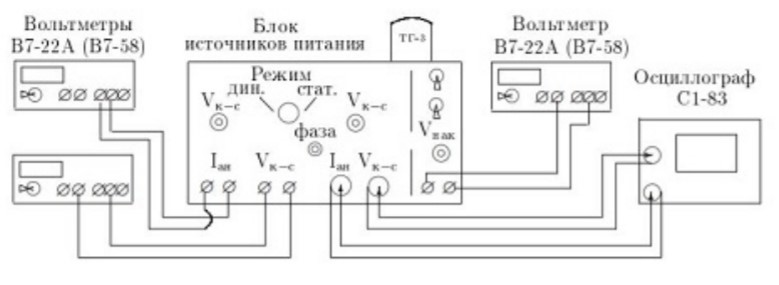
\includegraphics[width = 0.6\textwidth]{3.jpg}
\caption{Блок-схема экспериментальной установки}
\end{center}
\end{figure}
\newpage
\section*{Ход работы}
Снимем с помощью осциллографа ВАХ при двух различных напряжениях, а затем померяем $V_{\max}$, $V_{\min}$ и $V_{\text{пробоя}}$ в зависимости от $U_{\text{накала}}$. Все данные, в том числе и изображения, занесем в таблицу.

% Please add the following required packages to your document preamble:
% \usepackage[table,xcdraw]{xcolor}
% If you use beamer only pass "xcolor=table" option, i.e. \documentclass[xcolor=table]{beamer}
\begin{table}[h]
\begin{center}
\begin{tabular}{|c|c|c|c|}
\hline
{\color[HTML]{333333} $U_{\text{накала}}$, В} & {\color[HTML]{333333} $V_{\max}$, В} & {\color[HTML]{333333} $V_{\min}$, В} & {\color[HTML]{333333} $V_{\text{пробоя}}$, В} \\ \hline
{\color[HTML]{333333} 3,041}                & {\color[HTML]{333333} 2,8}        & {\color[HTML]{333333} 6,84}        & {\color[HTML]{333333} 12,0}                  \\ \hline
{\color[HTML]{333333} 2,75}                & {\color[HTML]{333333} 2,8}        & {\color[HTML]{333333} 6,6}          & {\color[HTML]{333333} 12,0}                  \\ \hline
{\color[HTML]{333333} $\sigma_U = 0,01$ В} & \multicolumn{3}{c|}{{\color[HTML]{333333} $\sigma_V = 0,4$ В}}                                                     \\ \hline
\end{tabular}
\caption{напряжения максимума, минимума и пробоя, в зависимости от накала}
\end{center}
\end{table}
Здесь погрешность для накала берем как $\Delta U_{\text{накала}} = 0,0015 U + 0,003$. Поскольку у нас немного плавали цифры, то можно погрешность округлить до $0,01$ В.
\begin{figure}[h]
\begin{center}
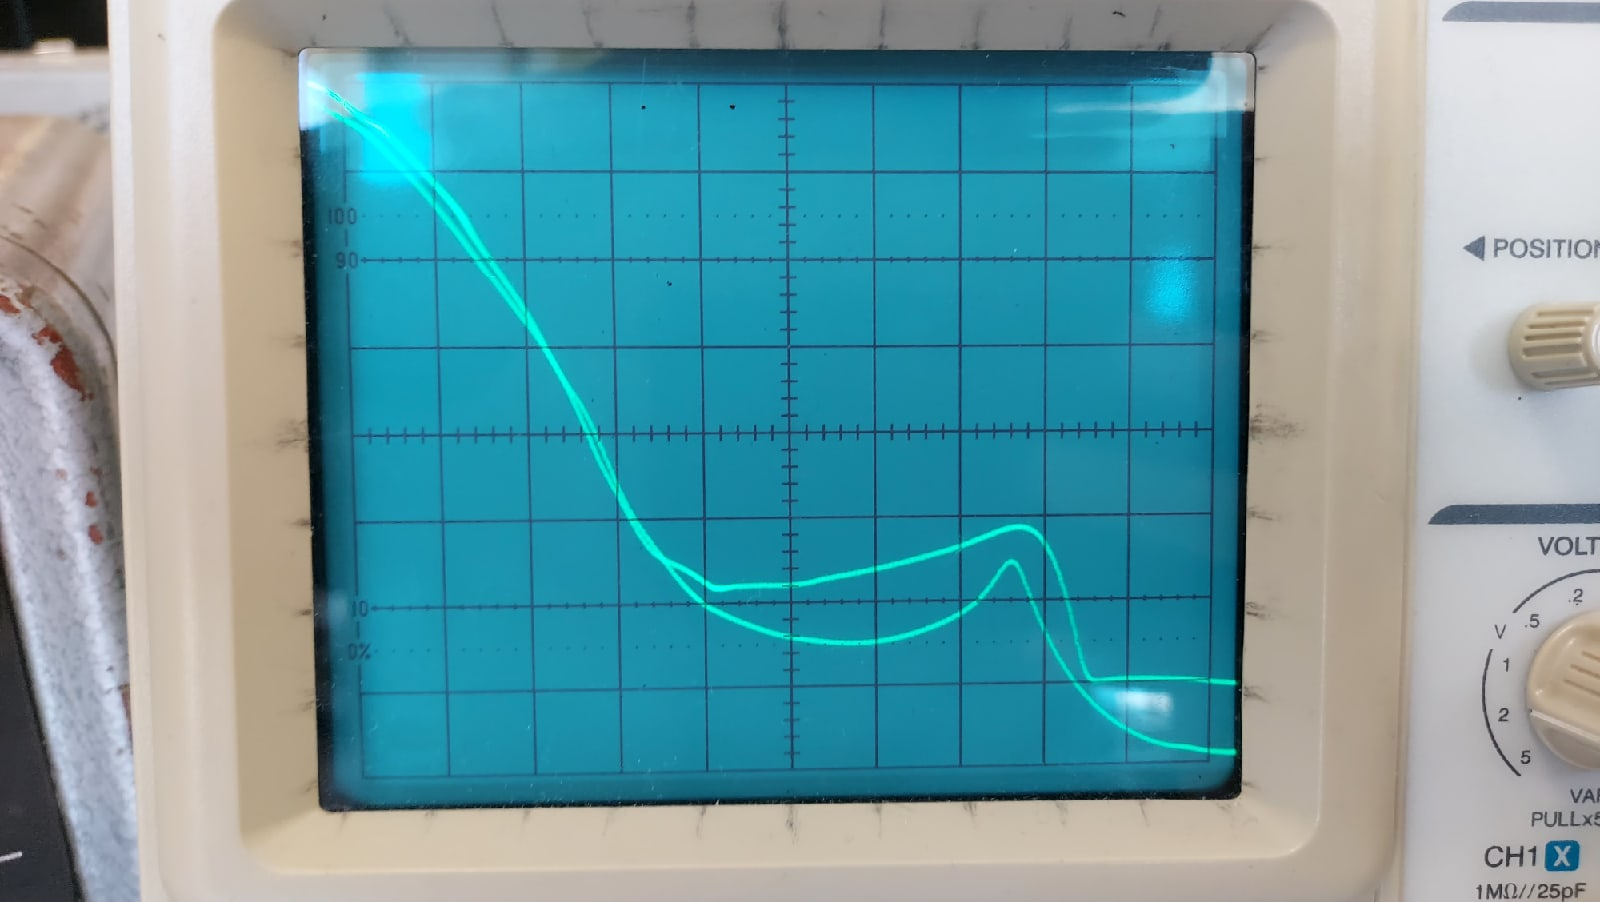
\includegraphics[width = 0.4\textwidth]{2.jpg}
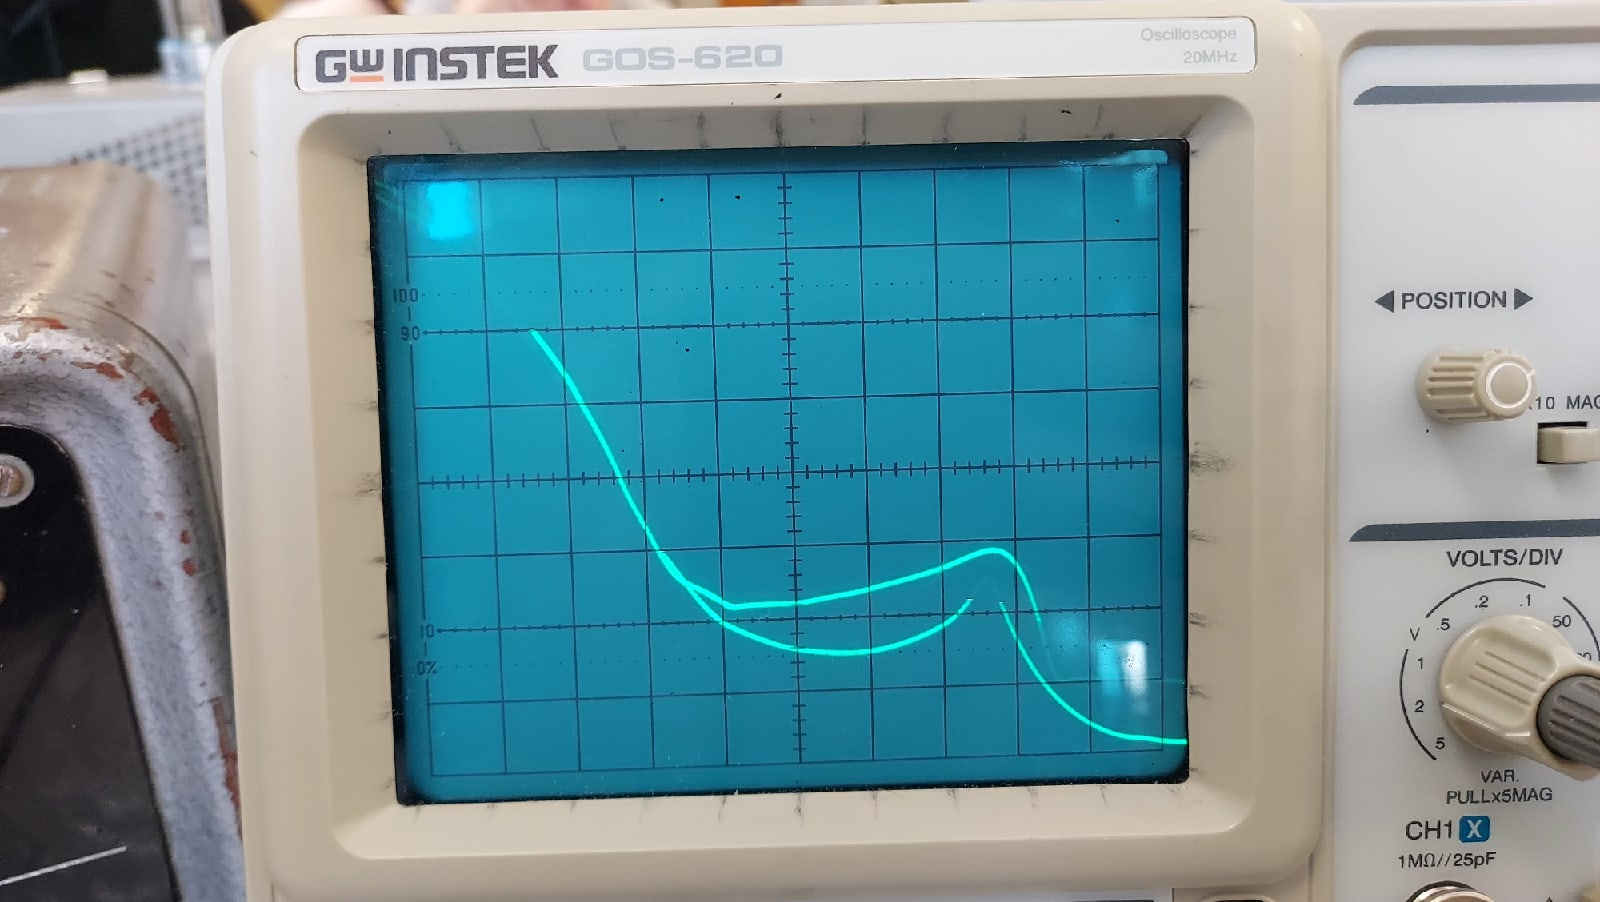
\includegraphics[width = 0.4\textwidth]{4.jpg}
\caption{Изображения кривой на осциллографе (слева для 3,04 В)}
\end{center}
\end{figure}

В развертке нас интересует только ось $Y$, по ней цена деления: $0,2$ В. Для напряжений увеличиваем погрешность в 2 раза, так как у нас не совпадают две кривые на осциллографе.

Теперь рассчитаем, для приведенных выше данных рассчитаем размер электронной оболочки атома, сделаем мы это из формул $(7)б (8)$.

В итоге мы получим систему из 2 уравнений: 
\begin{equation}
\left\lbrace \begin{array}{l}
2l = \dfrac{h}{\sqrt{2m(E_1 + U_0)}}\\
 \\
2l = \dfrac{3}{2}\dfrac{h}{\sqrt{2m(E_2 + U_0)}} 
\end{array} \right.
\end{equation}

А поскольку мы принимаем $U_0 = 2,5$ В, а $E_1$ и $E_2$ можно легко получить, домножив соответствующие $V$, которые мы померяли на $e$. 

К сожалению этот метод не даст нужных результатов, поскольку если посчитать эту систему с предположением, что $U_0 = 2,5$ В для $U_\text{накала} = 3,04$ В, то получится
\[
\left\lbrace \begin{array}{l}
2l = (5,3\pm 0,5) \text{В}\\
2l =  (6,04 \pm 0,11) \text{В}
\end{array} \right.
\]

Это связано с тем, что глубина ямы на самом деле намного меньше, мы можем просто ее посчитать по формуле $(8)$ и получить, что 

\[U_0 = (0,4 \pm 0,1) eV\]

Здесь, выше и далее мы считаем погрешность, как погрешность сложной функции, то есть через корень суммы частных производных на относительную погрешность в квадрате.
Поэтому мы считаем $l$ по формуле $(7)$ и получаем
\[l = (3,4 \pm 0,4) \text{\AA}\]

Во всех наших измерениях, поскольку наши кривые не совпадают, имеет смысл завысить погрешность, поскольку были проблемы.

Приведем таблицу, с итоговыми данными $U_0$ и $l$ для обоих $U_{\text{накала}}$

\begin{table}[h]
\begin{center}
\begin{tabular}{|c|c|c|}
\hline
$U_{\text{накала}}$ & $l$, \AA & $U_0, eV$     \\ \hline
3,04                & $3,4\pm0,4$             & $0,4\pm0,1$ \\ \hline
2,75                & $3,5\pm0,5$             & $0,3\pm0,1$ \\ \hline
\end{tabular}
\caption{Зависимость $l$ и $U_0$ от накала}
\end{center}
\end{table}
Далее оценим ионизационный потенциал, который получается так:
\[U = U_0 + U_{\text{пробоя}} \approx 12,3 \pm 0,4 \text{В}\]

Значит мы имеем дело в данной работе со ксеноном.

Далее проделаем то же самое, только для ВАХа. Далее последуют только графики и таблицы, поскольку порядок действий уже обговорен далее.
\begin{figure}[h]
\begin{center}
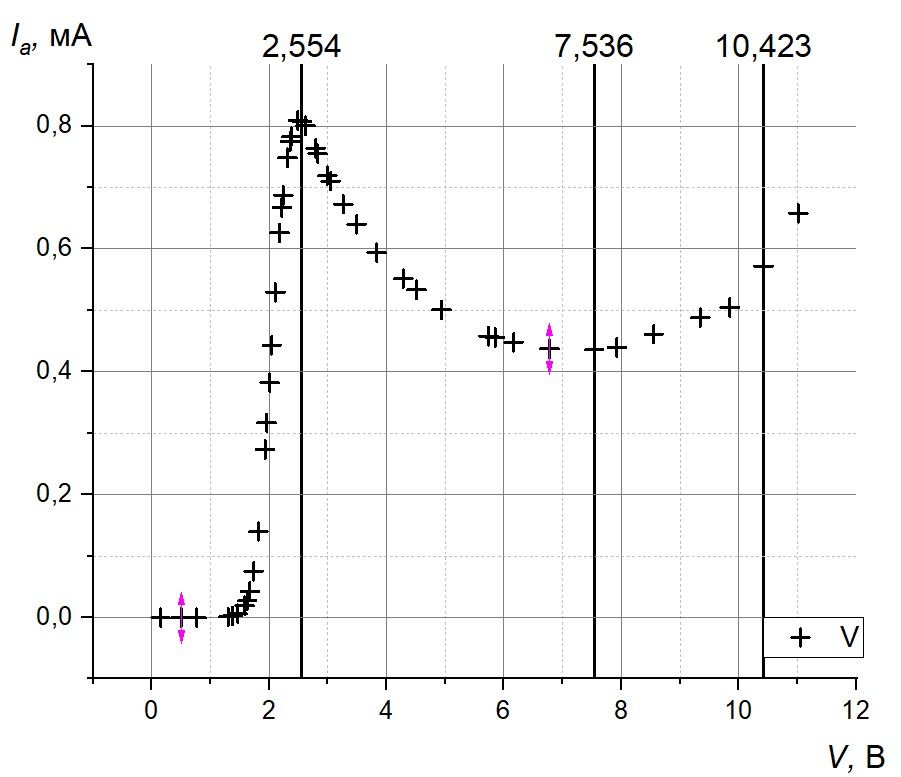
\includegraphics[width = 0.7\textwidth]{5.jpg}
\caption{ВАХ для $U_{\text{накала}} = 3,04$ В}
\end{center}
\end{figure}
\newpage
\begin{figure}[h]
\begin{center}
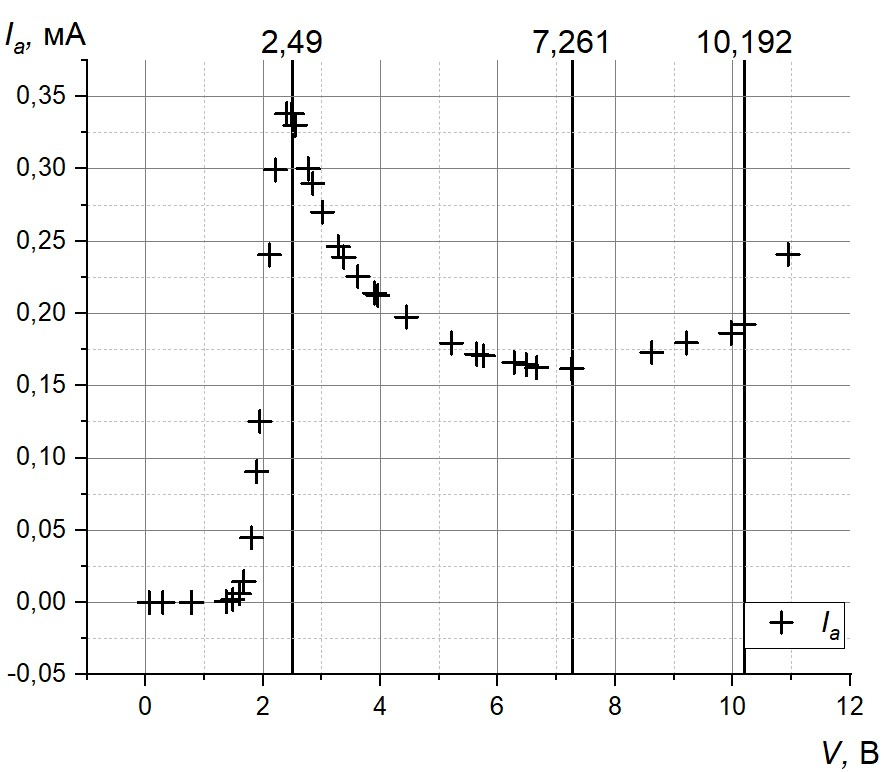
\includegraphics[width = 0.7\textwidth]{6.jpg}
\caption{ВАХ для $U_{\text{накала}} = 2,75$ В}
\end{center}
\end{figure}
% Please add the following required packages to your document preamble:
% \usepackage[table,xcdraw]{xcolor}
% If you use beamer only pass "xcolor=table" option, i.e. \documentclass[xcolor=table]{beamer}
\begin{table}[h]
\begin{center}
\begin{tabular}{|c|c|c|c|}
\hline
$U_{\text{накала}}$ &  $V_{\max}$ &  $V_{\min}$ &  $V_{\text{пробоя}}$ \\ \hline
3,04                & 2,6                               & 7,5                               & 10,4                                       \\ \hline
2,75                & 2,5                               & 7,3                               & 10,2                                       \\ \hline
$\sigma_U = 0,01$ В & \multicolumn{3}{c|}{$\sigma_V = 0,1$ В}                                                                            \\ \hline
\end{tabular}
\caption{разные напряжения для статического метода}
\begin{tabular}{|c|c|c|}
\hline
$U_{\text{накала}}$ & $l$, \AA & $U_0, eV$     \\ \hline
3,04                & $3,1\pm0,2$             & $1,32\pm0,03$ \\ \hline
2,75                & $3,1\pm0,3$             & $1,34\pm0,02$ \\ \hline
\end{tabular}
\caption{Финальные данные для статического метода}
\end{center}
\end{table}

Найдем зависимость $E_n(E_1, n)$, используя формулу 
\[\sqrt{\frac{2m(E_n + U_0)}{\hbar^2}}l = \pi n\]	

В итоге получаем, что 
\[E_n = n^2(E_1 + U_0) - U_0\]
Отсюда при $E_2 = 14,0 eV, E_3 = 33,1 eV, E_4 =59,8 eV$ 

При таких энергиях электронов происходит ионизация газа, из-за чего наступает пробой и уже второй максимум измерить не удается.

На основе формулы $(9)$ мы можем построить график зависимости вероятности рассеяния электрона от ускоряющего напряжения.
\newpage
\begin{figure}[h]
\begin{center}
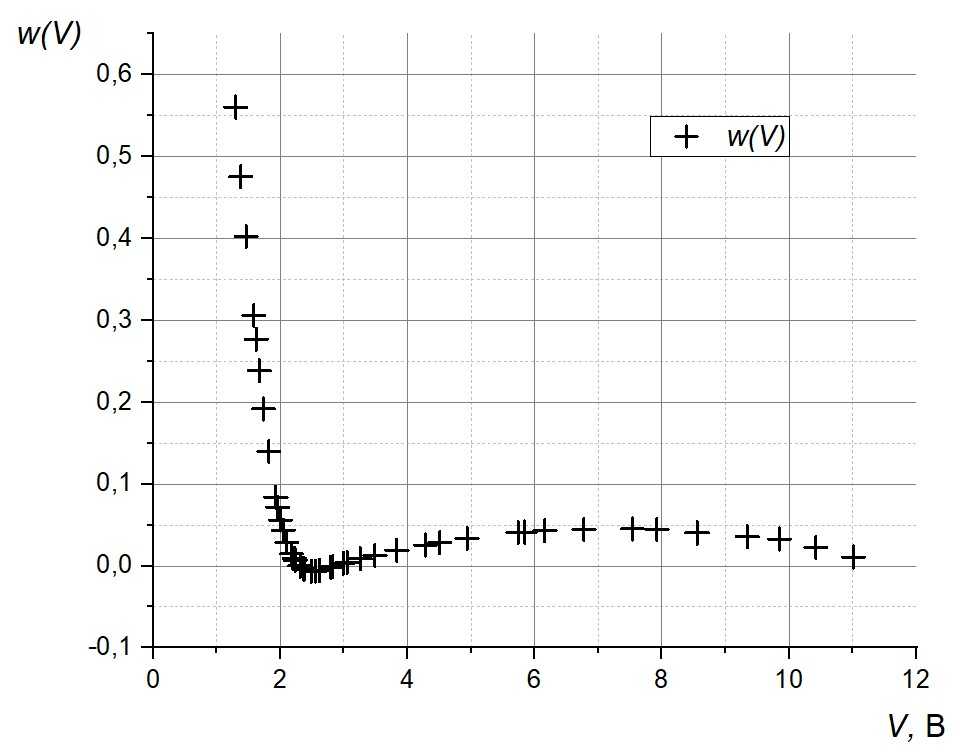
\includegraphics[width = 0.8\textwidth]{7.jpg}
\caption{Зависимость $w(V)$}
\end{center}
\end{figure}
\section*{Вывод}
Мы провели опыты по изучению рассеяния медленных электронов и получили верные ВАХ динамическим и статическим методами. Так же мы выяснили, что в нашей установке был ксенон.
\end{document}
